\documentclass[12pt]{extarticle}
\usepackage[english]{babel}
\usepackage{graphicx}
\usepackage{framed}
\usepackage[normalem]{ulem}
\usepackage{amsmath}
\usepackage{amsthm}
\usepackage{amssymb}
\usepackage{amsfonts}
\usepackage{enumerate}
\usepackage[utf8]{inputenc}
\usepackage[top=1 in,bottom=1in, left=1 in, right=1 in]{geometry}
\usepackage{graphicx}
\usepackage[skip=2pt]{caption}
\captionsetup{font={small}} 
\graphicspath{{Figuras/}}
\usepackage{appendix}
\newcommand{\asp}[1]{``#1"}
\usepackage[colorinlistoftodos]{todonotes}
\newcommand{\nota}[1]{\todo[color=black!10, bordercolor=white!100, linecolor = black!20, size =\scriptsize]{#1} }
\definecolor{mypink1}{rgb}{0.858, 0.188, 0.478}
\definecolor{mypink2}{RGB}{219, 48, 122}
\definecolor{mypink3}{cmyk}{0, 0.7808, 0.4429, 0.1412}
\definecolor{mygray}{gray}{0.6}
\newcommand{\arb}{um elemento arbitrário }
\newenvironment{resposta}{ \color{mygray}}{}
\newcommand{\true}{\textcolor{red}{\textbf{\textit{V}}}}
\newcommand{\false}{\textcolor{red}{\textbf{\textit{F}}}}
\newcommand{\keys}[1]{\{#1\}}
\newenvironment{direta}{}{
\begin{flushright}
    Q.E.D
\end{flushright}
}
\newenvironment{contradicao}{A prova é por contradição.}{
\begin{flushright}
    Q.E.D
\end{flushright}
}
\newenvironment{contrapositiva}{A prova é pela contrapositiva.}{
\begin{flushright}
    Q.E.D
\end{flushright}
}
\newcommand{\definition}[3][x]{\{#1|#1 \in \mathbb{#2},#3\}}
\newcommand{\natura}{\mathbb{N}}
\newcommand{\integer}{\mathbb{Z}}
\newcommand{\real}{\mathbb{R}}
\newenvironment{pif}[3][1]{
Tomando $n = #1$ então $#2$ e $#3$

Agora vamos assumir que a expressão é valida para $#1 > n \leq k$ e vamos provar que funciona para $n=k+1$.
}{}
\newcommand{\arranjo}[2]{A_{#1,#2}=\frac{#1!}{(#1-#2)!}}
\newcommand{\arranjoform}[2]{\frac{#1!}{(#1-#2)!}}
\newcommand{\conbination}[2]{C_{#1,#2}=\frac{#1!}{#2!(#1-#2)!}}
\newcommand{\conbinationform}[2]{\frac{#1!}{#2!(#1-#2)!}}
\newcommand{\rconbination}[2]{CR_{#1,#2}=\frac{(#1+#2-1)!}{#2!(#1-1)!}}
\newcommand{\clinear}[1]{\foreach \i in {1,...,#1}{x_\i+}}
\newcommand{\fatorial}[2]{\foreach \i in {#1,...,#2}{\i.}}
\newcommand{\soma}[2]{\sum_{n=#1}^{\infty}#2}
\usepackage{blindtext}
\newcommand{\texto}{\color{mygray}\blindtext\color{black}}



%--------------%--------------%----------------------%-----------%--------------

\title{Projeto Wikiaves (WAV) x SpeciesLink (SLI)}
\author{Universidade Federal do ABC}
\date{Novembro, 2020}

\begin{document}


\maketitle

%\textbf{Considerações}
%\begin{enumerate}
%\item 
%\end{enumerate}
%\newpage

\section{Análise Univariada}

\hrulefill

Como escrever \asp{Média (Desvio Padrão) retro-transformados} acaba ficando muito grande na tabela, deixei uma linha abaixo do \asp{bloco} Log10 para a retro-transformação, em particular acho que não ajudou muito, porém, não sei se deixar apenas \asp{retro-transformação} seria o ideal. Na seção 2 fica ainda mais esquisito (esteticamente falando).

\hrulefill


\begin{resposta}
Os sítios Wikiaves e SpeciesLink são bases de dados distintas que contam com registros de espécies de aves. No estado de São Paulo, a capacidade amostral varia de acordo com sítio analisado, o Wikiaves, cobre 631 dentre os 645 municípios do estado e, o SpeciesLink, cobre 174. Ao valer-se apenas dos municípios registrados em ambas as bases de dados, há apenas uma que aparece exclusivamente no SpeciesLink, esta cidade, por sua vez, não possuí grande influência sob os valores restantes da amostra. 

Por este motivo as análises conduzidas se dividirão em 3 categorias: Wikiaves, SpeciesLink e Wikiaves valendo-se apenas dos 173 municípios que possuem registros em ambas as bases.

\end{resposta}

\begin{figure}[h!]
\centering
{\scriptsize Tabela 1: Número de registros, espécies e municípios em cada banco de dados.}
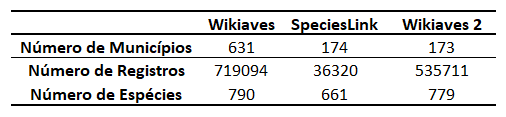
\includegraphics{Imagens/T01.png}
\end{figure}

\begin{resposta}
Em sequencia, serão abordadas as variáveis de registros por município, espécies por município e registros por espécie.
\end{resposta}

\subsection{Registros por Município}

\begin{resposta}
As medidas de tendencia central e dispersão para o número de registros por município encontram-se na tabela a seguir: 
\end{resposta}

\begin{figure}[h!]
\centering
{\scriptsize Tabela 2: Estatísticas de tendência central e dispersão para o número de registros em cada banco de dados.}
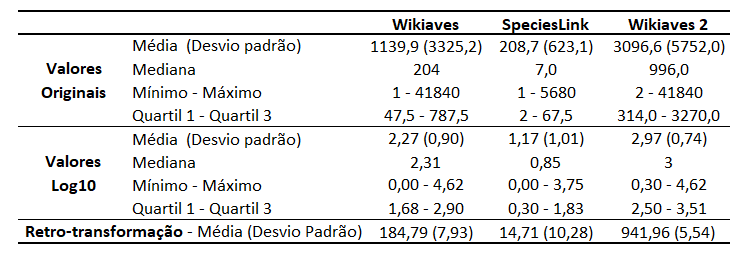
\includegraphics{Imagens/T02.png}
\end{figure}

\newpage

\begin{resposta}
A quantidade de registros no Wikiaves é uma ordem de grandeza maior que a do SpeciesLink. Embora as disparidades não sejam tão evidentes, a média de registro por município acompanha este padrão. Entretanto, esse tópico traz uma mediana que é, no mínimo, cinco vezes menor que a média para ambas as bases analisadas, este fato, acrescido das distâncias distintas entre os quartis justificam o desvio padrão, que vale cerca de três vezes a média. Isto sugere que a distribuição de registros por município não é homogenia quando exploradas as variáveis originais. Para que os valores sejam significativos, aplica-se uma transformação logarítmica cujos valores estão, igualmente, dispostos na tabela. A desproporção entre as médias dos bancos de dados é maior na relação SpeciesLink - Wikiaves 2, também este possui cerca de quatorze vezes a quantidade de registros por município que o SpeciesLink. Quando analisados os quartis, a disparidade entre os sítios aumenta, bem como para a mediana. 

Após a transformação, percebe-se que os valores para o SpeciesLink permanecem não uniformes, contudo, mais uniformes que anteriormente. O Wikiaves, por outro lado, apresenta-se de forma quase homogenia, a distância entre a média e a mediana é de 0,16, isso representaria 1,44 em valores não logarítmicos, contrastando com a distância de 935,6 obtida pelas variáveis originais, ademais, o desvio padrão neste sítio é menor que o do SpeciesLink, embora o Wikiaves possua valores maiores. De fato, o Wikiaves assemelha-se a uma curva de sino, vez que, o SpeciesLink apresenta um decaimento.

Espero que você não esteja lendo isto, usei o blindtext pra tampar o espaço que ficava aqui \blindtext 

\end{resposta}

\newpage

\begin{figure}[h!]
\centering
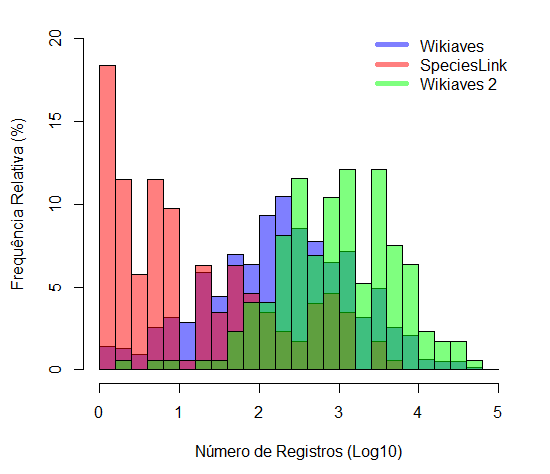
\includegraphics[height = 8cm]{Imagens/H01.png}
\\{\scriptsize Figura 1: Frequência relativa (\%) do número de registros (log10) pelo número de municípios, respetivamente, 631,174 e 173 para os Wikiaves, SpeciesLink e Wikiaves2  }
\end{figure}

\subsection{Espécies por Município}

\begin{resposta}
As medidas de tendencia central e dispersão para a categoria de espécies por município encontram-se na tabela a seguir: 
\end{resposta}


\begin{figure}[h!]
\centering
{\scriptsize Tabela 3: Estatísticas de tendência central e dispersão para o número de espécies em cada banco de dados.}
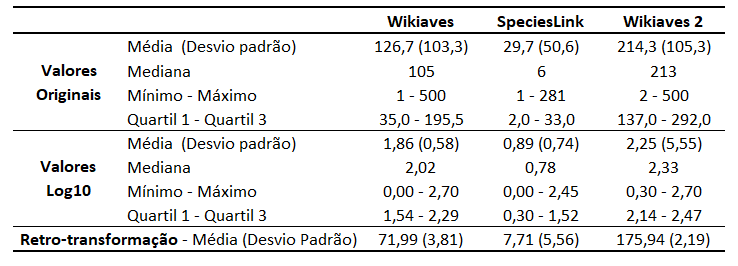
\includegraphics{Imagens/T03.png}
\end{figure}

\begin{resposta}
Há 202 espécies que possuem registro apenas no Wikiaves, enquanto 73 possuem registros apenas no SpeciesLink, os bancos de dados contam com 790 e 661 espécies, respectivamente. A média de espécies por município é, no mínimo, quatro vezes maior para o Wikiaves, é notável que, para tal, o primeiro quartil é maior que o terceiro quartil de seu oposto. Embora isto, a distância entre a média e a mediana é menor nesta base, bem como, o desvio padrão é o dobro em relação à outra, estes valores indicam um padrão mais próximo de uma curva de sino, não obstante, há a necessidade da transformação logarítmica para padronizar os dados do SpeciesLink.

Dentre as 790 espécies que constam no Wikiaves para o estado de São Paulo, 779 possuem registros nos 173 municípios desta análise. O Wikiaves demonstra valores maiores para todos os campos, a distância entre a média e a medina é menor que na seção anterior, os quartis apresentam distância similares entre si, contudo, ainda não são uniformes. É razoável concluir que o Wikiaves apresenta um padrão próximo ao de sino, mesmo para as variáveis originais.

Após transformados, os dados tornam-se mais homogêneos para o SpeciesLink, como esperado, porém ainda não chegam a um padrão. Para o Wikiaves, a mediana torna-se maior que a média, indicando que, de fato, o padrão anterior também se aproxima de uma curva uniforme.

Aplica-se a transformação logarítmica para seguir o procedimento aplicado ao SpeciesLink. Com isto, a mediana para o Wikiaves torna-se maior que a média, a distância entre os quartis é, de certa forma, regular. Contudo, a distância entre o valor mínimo e o primeiro quartil é quase quatro vezes a distância entre o terceiro quartil e o valor máximo.

O SpeciesLink, por certo, não apresenta padrão de sino, por outro lado, o decaimento observado seria maior para as variáveis originais. O Wikiaves está mais próximo deste padrão, distingui-se por, no lugar de decaimento, apresentar uma curva crescente com uma queda intensa ao final.
\end{resposta}



\begin{figure}[h!]
\centering
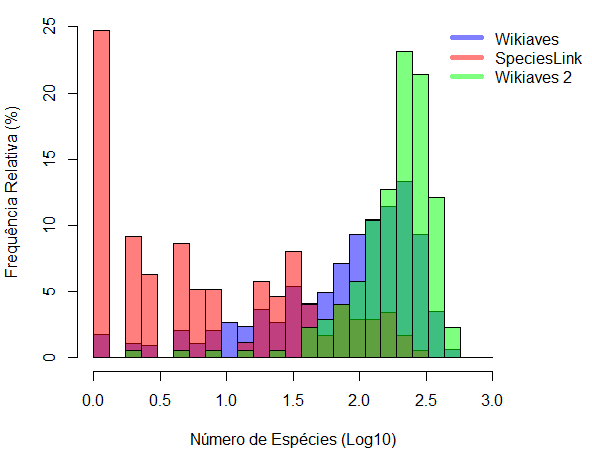
\includegraphics[height = 8cm]{Imagens/H02.png}
\\{\scriptsize Figura 2:Frequência relativa (\%) do número de espécies (log10) pelo número de municípios, respetivamente, 631,174 e 173 para os Wikiaves, SpeciesLink e Wikiaves2  }
\end{figure}


\subsection{Registros por Espécie}

\begin{resposta}
As medidas de tendencia central e dispersão para a categoria de registros por espécie encontram-se na tabela a seguir: 
\end{resposta}

\newpage

\begin{figure}[h!]
\centering
{\scriptsize Tabela 4: Estatísticas de tendência central e dispersão para o número de registros por espécie em cada banco de dados.}
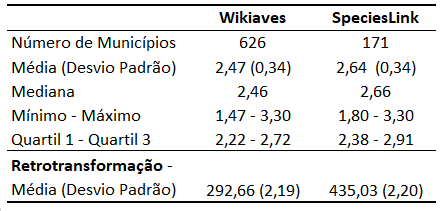
\includegraphics{Imagens/T04.png}
\end{figure}


\begin{resposta}
Para registros por espécie, além da quantidade de registros, a média e a mediana, também, são de uma ordem de grandeza maior para o Wikiaves. Neste, a média é quase o dobro da mediana e o desvio padrão é, inclusive, maior que a média. A distância entre os quartis não é regular para ambos os bancos de dados, no SpeciesLink, a média é maior que o terceiro quartil e o desvio padrão é, no mínimo, quatro vezes a média. Ambos não apresentam um padrão de sino, portanto, aplica-se a transformação logarítmica a fim de uniformizar esses dados. O Wikiaves 2 não se distingue do que foi descrito.

Após a transformação a mediana ultrapassa a média, em ambos, contudo, mais próxima. A distância entre os quartis é mais regular, porém, ainda não é uniforme. No Wikiaves, a distância entre o primeiro quartil e o mínimo é mais em relação à distância entre o terceiro e o máximo. No SpeciesLink, ocorre o oposto, a distância entre o primeiro quartil e o número mínimo é menor que a distância entre o terceiro quartil e o número máximo.
 
\end{resposta}

\begin{figure}[h!]
\centering
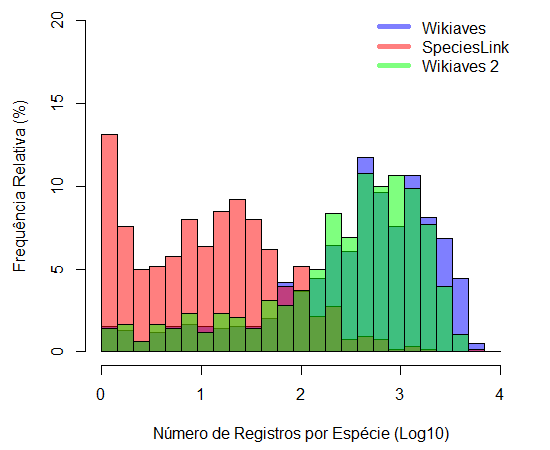
\includegraphics[height = 8cm]{Imagens/H03.png}
\\{\scriptsize Figura 3: Frequência relativa (\%) do número de registros (log10) pelas número de registros (log10).}
\end{figure}

\newpage

\section{Fatores Externos}

\begin{resposta}
Em cada seção será apresentada a tabela correspondente aos valores de tendencia central e dispersão para cada varável. Para as analises posteriores serão excluídos os outliers mencionados nesta. Os parâmetros de latitude e longitude são os únicos que não apresentam outliers.
\end{resposta}


\subsection {Altitude}

\begin{figure}[h!]
\centering
{\scriptsize Tabela 5: Estatísticas de tendência central e dispersão para altitude em metros.}
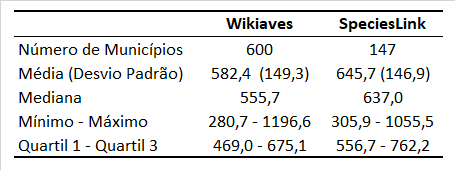
\includegraphics{Imagens/T05.png}
\end{figure}


\begin{resposta}
A Altitude para o Wikiaves apresenta média menor, isto é, as cidades excedentes nesta base, em sua maioria, estão a altitudes mais baixas que a média do SpeciesLink. De fato, o mesmo ocorre para a mediana e os quartis. Foram excluidos os valores maiores e menores que 1200 e 200, respetivamente. Pelos histogramas é possível notar que os bancos de dados apresentam uma quantidade similar de outliers. 
\end{resposta}



\begin{figure}[h!]
\centering
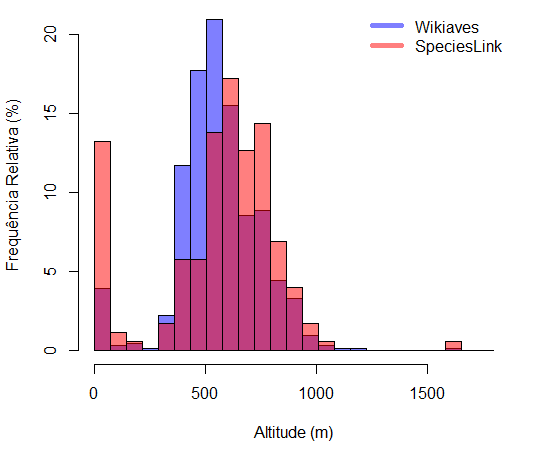
\includegraphics[height = 8cm]{Imagens/H04.png}
\\{\scriptsize Figura 4: Distribuição de altitude (em metros) em cada base. Foram excluídos da análise os municípios abaixo de 250 ou acima de 1200.}
\end{figure}

\newpage

\subsection{Área}

\begin{figure}[h!]
\centering
{\scriptsize Tabela 6: Estatísticas de tendência central e dispersão para área em $\log_{10}(\text{Km}^2)$.}
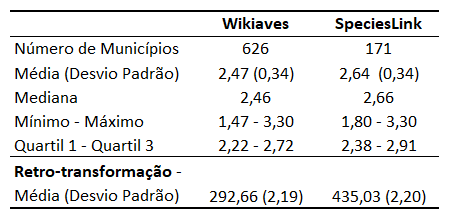
\includegraphics{Imagens/T06.png}
\end{figure}

\begin{resposta}
Observa-se que a média e a mediana ficam próximas, o desvio padrão também é baixo, em relação à análise da seção 1. Foram excluidos os outliers menores que 1,4.
\end{resposta}



\begin{figure}[h!]
\centering
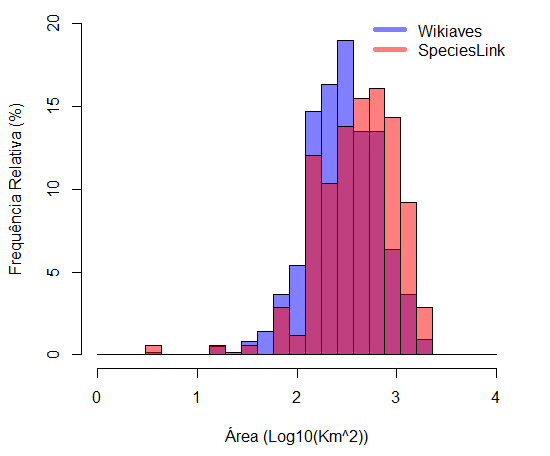
\includegraphics[height = 8cm]{Imagens/H05.png}
\\{\scriptsize Figura 5: Distribuição de área (em $\log_{10}(\text{Km}^2)$)em cada base. Foram excluídos da análise os municípios menores que 1,4 para o Wikiaves e 1,6 para o SpeciesLink. }
\end{figure}

\newpage

\subsection{População}

\begin{figure}[h!]
\centering
{\scriptsize Tabela 7: Estatísticas de tendência central e dispersão para o número de habitantes por município.}
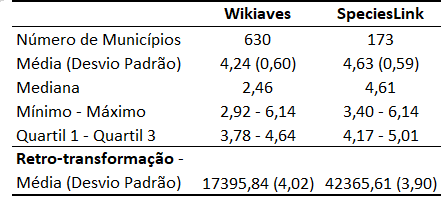
\includegraphics{Imagens/T07.png}
\end{figure}

\begin{resposta}
A média do Wikiaves é menor que a do SpeciesLink, bem como a mediana e os quartis, isto é, o Wikiaves cobre mais cidades menos habitadas. Os dados do SpeciesLink apresentam-se um pouco mais homogêneos, contudo, ambos seguem uma curva de sino quando excluído o mesmo outlier, 7.
\end{resposta}


\begin{figure}[h!]
\centering
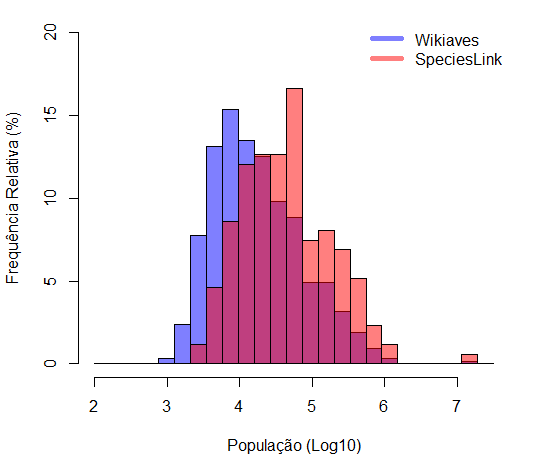
\includegraphics[height = 8cm]{Imagens/H06.png}
\\{\scriptsize Figura 6: Distribuição populacional (Log10) de em cada base. Foram excluídos da análise o município maior que 6,5.}
\end{figure}

\newpage

\subsection{Latitude}

\begin{figure}[h!]
\centering
{\scriptsize Tabela 8: Estatísticas de tendência central e dispersão para latitude em graus.}
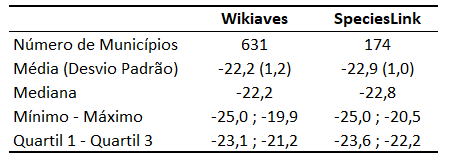
\includegraphics{Imagens/T08.png}
\end{figure}

\begin{resposta}
A princípio as bases de dados possuem uma curva muito parecida, entretanto, para municípios em latitudes mais altas o Wikiaves se sobressai. Os quartis são regulares e o desvio padrão é baixo. 
\end{resposta}

\begin{figure}[h!]
\centering
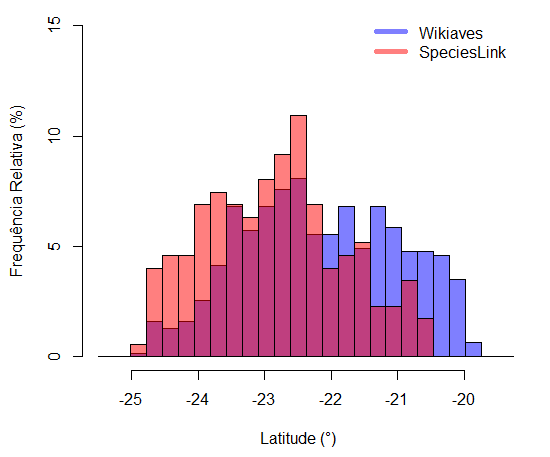
\includegraphics[height = 8cm]{Imagens/H07.png}
\\{\scriptsize Figura 7: Distribuição de latitude (em graus) de acordo com os municípios registrados em cada base.}
\end{figure}

\newpage

\subsection{Longitude}


\begin{figure}[h!]
\centering
{\scriptsize Tabela 9: Estatísticas de tendência central e dispersão para longitude em graus.}
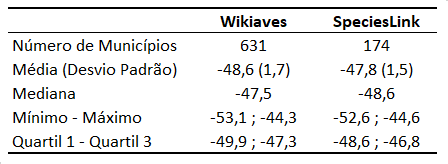
\includegraphics{Imagens/T09.png}
\end{figure}

\begin{resposta}
O Wikiaves possui mais cidades em longitudes mais baixas, além disto, sua média é igual à mediana e o desvio padrão é baixo, com intervalo quase regular entre os quartis. Para o SpeciesLink, o padrão de baixo desvio padrão se mantém, mas, a regularidade da distância dos quartis é menor.
\end{resposta}


\begin{figure}[h!]
\centering
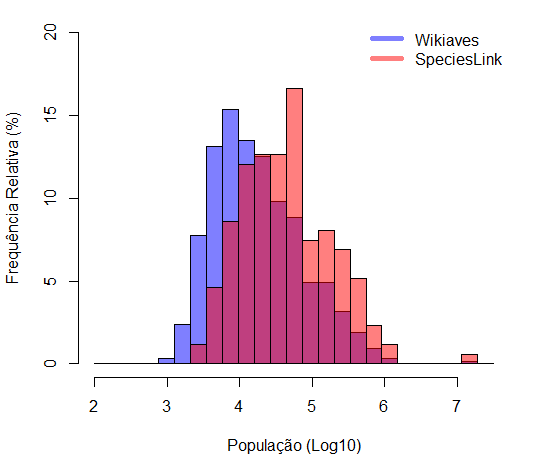
\includegraphics[height = 8cm]{Imagens/H06.png}
\\{\scriptsize Figura 7: Distribuição de longitude (em graus) de acordo com os municípios registrados em cada base.}
\end{figure}

\newpage

\section{Análise Bivariada}

\hrulefill

Na última reunião você falou algo sobre a quantidade de municípios e eu comentei sobre os municípios sobrepostos. Então, pensei sobre e vi que havia uma falha na maneira com a qual eu estou representado os gráficos. Eu coloquei os municípios do WAV2 em uma camada acima do WAV, assim espera-se que todos os pontos verdes sejam também pontos vermelhos (WAV2 está sobreposto ao WAV). 

Acontece que isto não é uma regra, como foi feita a exclusão de outliers bivariados em alguns gráficos há municípios que são outilers bivariados no WAV e não são outliers bivariados no WAV2. Quando eu coloco um grau de transparência nos pontos (assim como são os histogramas) é possível observar isto:

\begin{figure}[h!]
\centering
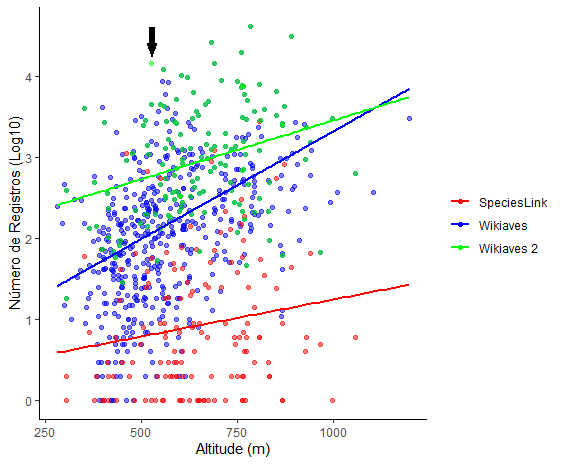
\includegraphics[height = 9cm]{Imagens/A.png}
\end{figure}

Por outro lado, o gráfico fica mais bagunçado. Por este motivo eu optei por intercalar os gráficos com o grau de transparência (registros) e aqueles sem o grau de transparência (espécies), assim o senhor pode avaliar qual é melhor.

O senhor também comentou rapidamente sobre a ANOVA. Para a análise de covariância partimos do pressuposto que os dados têm correlação linear (Gotelli), como em alguns pares de variáveis temos valores altos de p (em outros embora sejam menos que 0,05, não sei se isto é o suficiente para rejeitar a hipótese nula). Tive medo de cometer um erro do tipo I ao partir para este tipo de análise.

Como partiremos para ela de qualquer modo, devo excluir os pares ordenados que apresentam valores-p altos? Se uma variável explanatória apresenta correlação apenas com o Wikiaves e não com o SpeciesLink (analogamente apresentar apenas com registros e não com espécies) devo excluir apenas aquele que não apresenta correlação ou os respectivos pares?

\hrulefill

\newpage

\subsection{Registros}

\begin{resposta}
Os valores de correlação, valor-p e número de municípios encontram-se na tabela a seguir:
\end{resposta}


\begin{figure}[h!]
\centering
{\scriptsize Tabela 10: Valores de número de municípios (n), correlação (r), valor-p (p) para a\\ variação entre o número de registros (Log10) e variáveis explanatórias. }
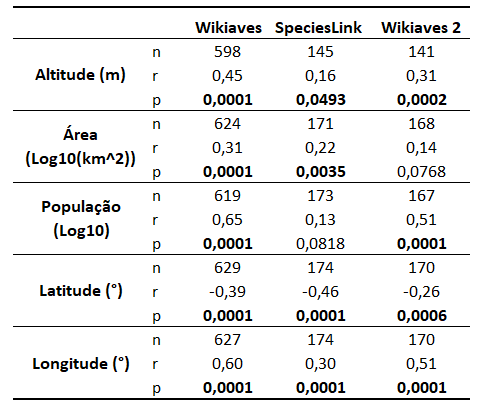
\includegraphics{Imagens/T10.png}
\end{figure}

 

\subsubsection{Altitude}

\begin{figure}[h!]
\centering
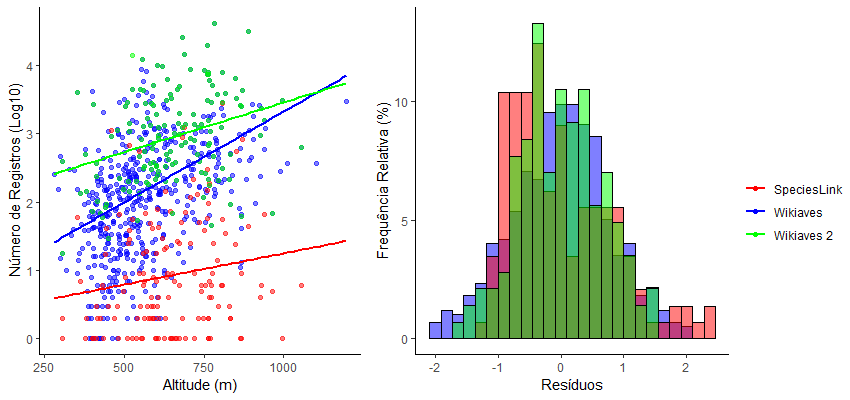
\includegraphics[width = 15cm]{Imagens/G01.png}
\\{\scriptsize Figura 8: Variação na quantidade de registros das bases conforme aumento de altitude e resíduos. Foram excluídos, 2 outliers bivariados no Wikiaves, 2 no SpeciesLink e 3 no Wikiaves 2. }
\end{figure}
\newpage

\begin{resposta}
Para o estado de São Paulo, embora hajam valores baixos de $p$ para o Wikiaves, o espaço amostral é de 598 municípios, portanto, espera-se que estes valores sejam pequenos. Para o SpeciesLink, a medida de $p$ que é maior que $0,01$, está próxima a este valor. O gráfico abaixo servirá de indicativo para determinar se a evidência coletada é o suficiente para a rejeição da hipótese nula.

De fato, a quantidade de registros no Wikiaves aumenta conforme o aumento de altitude. Contudo, não é um aumento evidente, há muitos pares ordenados distantes da reta, isto é, a reta de regressão neste caso não é uma boa aproximação para esta curva. Para o SpeciesLink, os gráficos explicitam que o valor de $p < 0,05$ e próximo a $0,01$ não é o suficiente para a rejeição da hipótese nula, na verdade, os dados mostram-se distantes da reta e sem padrão definido.

Quanto aos municípios registrados em ambos os bancos de dados, percebe-se, no Wikiaves, um aumento relevante do valor de $p$, que pode ser explicado pela diminuição da quantidade de cidades. 
\end{resposta}



\subsubsection{Área}


\begin{figure}[h!]
\centering
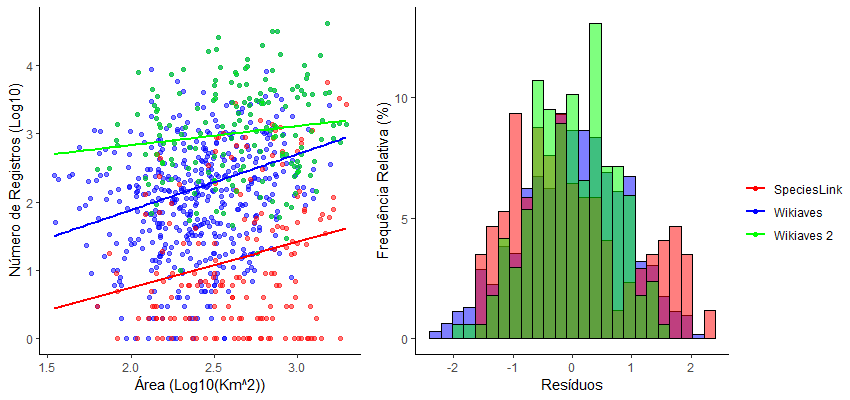
\includegraphics[width = 15cm]{Imagens/G02.png}
\\{\scriptsize Figura 9: Variação na quantidade de registros das bases conforme aumento de área e resíduos. Foram excluídos  2 outliers bivariados no Wikiaves 2.}
\end{figure}

\begin{resposta}
 Os valores de correlação linear para os municípios registrados no Wikiaves ou no SpeciesLink são de $0,31$ e $0,22$, respectivamente. Devido aos baixos valores de $p$ é possível que haja uma correlação não linear entre o que analisando, para confirmar ou contestar isto, atente-se ao gráfico: 
 
 É relevante que não há outliers bivariados. Além disto, há, de fato, um aumento linear, apesar disto, os pares ordenados encontram-se dispersos da reta de regressão, o que explica os baixos valores de correlação.

Ao diminuir a quantidade de cidades no Wikiaves, os valores de $p$ aumentam, torna-se maior que $0,01$, seguidos de valores baixos de $r$ em ambos. 

De fato, é possível afirmar que este parâmetro não possui grande influência sobre a quantidade de registros nas duas bases.
\end{resposta}



\subsubsection{População}

\begin{figure}[h!]
\centering
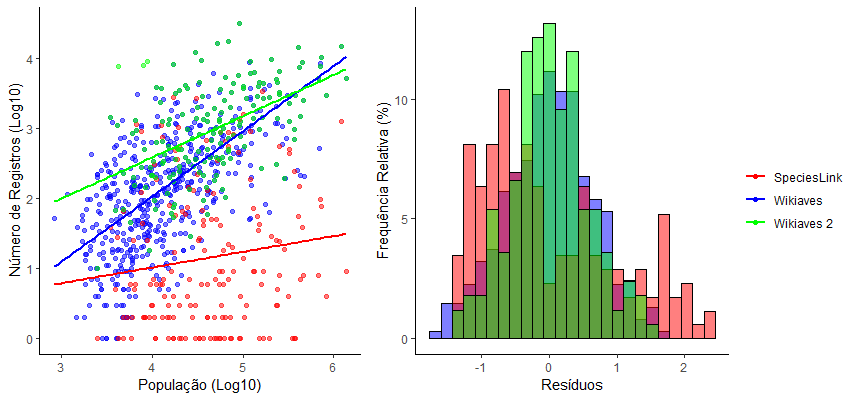
\includegraphics[width = 15cm]{Imagens/G03.png}
\\{\scriptsize Figura 10: Variação na quantidade de registros das bases conforme aumento da quantidade de habitantes e resíduos. Foram excluídos, 11 outliers bivariados no Wikiaves, 5 no Wikiaves 2.}
\end{figure}

\begin{resposta}
 O valor de correlação para os 619 municípios analisados para o Wikiaves é o maior obtido até então: $0,65$, um forte indicativo que há correlação linear nesta base. Em contrapartida, o SpeciesLink apresenta $p = 0,08$, que é um valor que exige cautela, como a correlação nesta base é de $0,13$ é possível assumir que não há correlação linear. Os gráficos a seguir confirmam isto.
 
\end{resposta}

\subsubsection{Latitude}

\begin{figure}[h!]
\centering
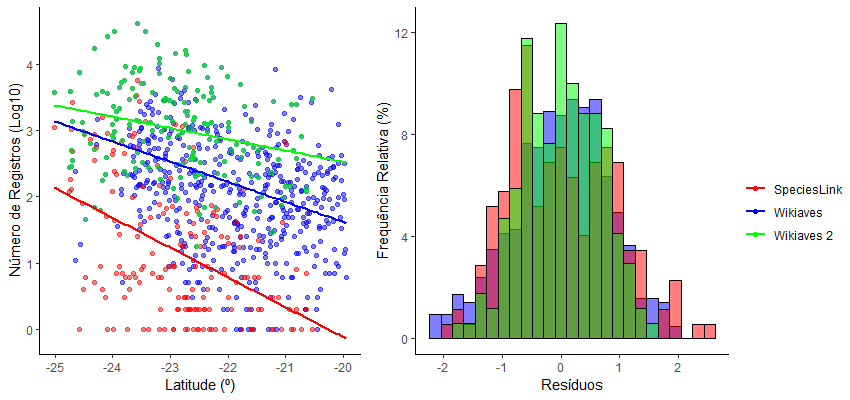
\includegraphics[width = 15cm]{Imagens/G04.png}
\\{\scriptsize Figura 11: Variação na quantidade de registros das bases conforme aumento de latitude e resíduos. Foram excluídos, 2 outliers bivariados no Wikiaves, 3 no Wikiaves 2.}
\end{figure}

\newpage

\begin{resposta}
 Os valores de $p$ e $r$, aparentam ser o suficiente para constatar que há um decaimento na quantidade de registros conforme aumento de altitude. 
 
 Os resíduos são regulares ao passo que estão dispersos da reta de regressão, há correlação linear, porém é baixa. Ao retirar as cidades excedentes os valores aumentam (no caso, o relacionamento é menor) no Wikiaves.
\end{resposta}

\subsubsection{Longitude}

\begin{figure}[h!]
\centering
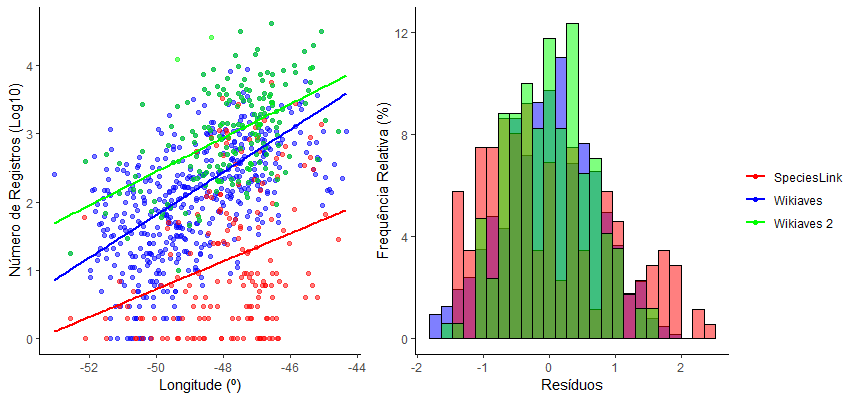
\includegraphics[width = 15cm]{Imagens/G05.png}
\\{\scriptsize Figura 12: Variação na quantidade de registros das bases conforme aumento de longitude e resíduos. Foram excluídos, 4 outliers bivariados no Wikiaves, 3 no Wikiaves 2.}
\end{figure}

 \begin{resposta}
O aumento linear é claro no Wikiaves e, embora não seja tão evidente assim, há um aumento no SpeciesLink, também.

Os resíduos regulares, bem como, o aumento no gráfico indicam que há relação.
\end{resposta}


\subsection{Espécies}

\begin{resposta}
Os valores de correlação, valor-p e número de municípios encontram-se na tabela a seguir:
\end{resposta}

\newpage

\begin{figure}[h!]
\centering
{\scriptsize Tabela 11: Valores de número de municípios (n), correlação (r), valor-p (p) para a\\ variação entre o número de espécies (Log10) e variáveis explanatórias.}
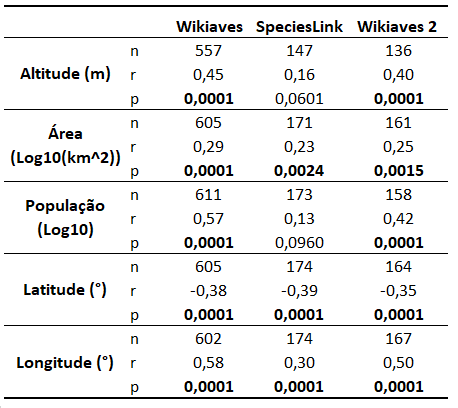
\includegraphics{Imagens/T11.png}
\end{figure}

\subsubsection{Altitude}


 

\begin{figure}[h!]
\centering
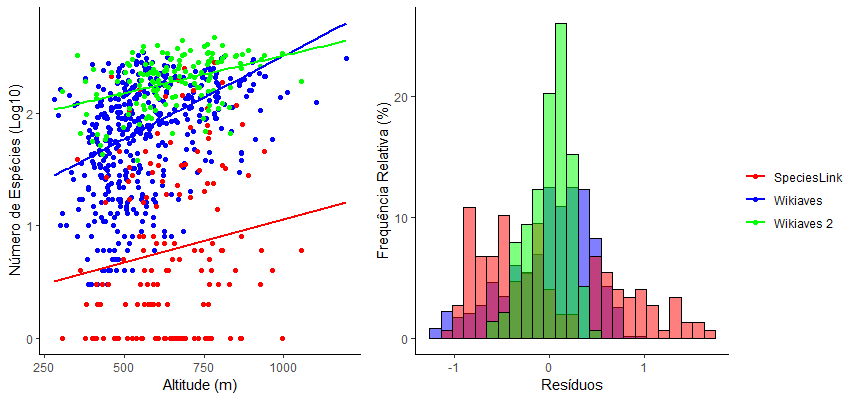
\includegraphics[width = 15cm]{Imagens/G06.png}
\\{\scriptsize Figura 13: Variação na quantidade de espécies das bases conforme aumento de altitude e resíduos. Foram excluídos, 23 outliers bivariados no Wikiaves, 8 no Wikiaves 2.}
\end{figure}


\begin{resposta}
Os valores de $p$ para a quantidade de espécies são, ainda, maiores que os que dizem respeito aos registros, neste cenário, é possível assumir que não há relação entre a altitude e os dados do SpeciesLink ($p > 0,05$). No caso da outra base, os valores de $p$ são baixos o suficiente para que haja relação. O gráfico abaixo explicita o comportamento. Novamente, os dados estão dispersos da linha de tendência no Wikiaves. No SpeciesLink, de fato, não há correlação linear.

Ao admitir apenas os 173 municípios registrados por ambas as bases, o valor de $p$ para o Wikiaves não sofre uma mudança tão drástica quanto para os registros, na verdade, este valor continua abaixo de $0,01$. Note, no gráfico abaixo, que os valores não estão dispersos da linha de tendência, portanto, pode assumir que há uma relação.
\end{resposta}

\subsubsection{Área}



\begin{figure}[h!]
\centering
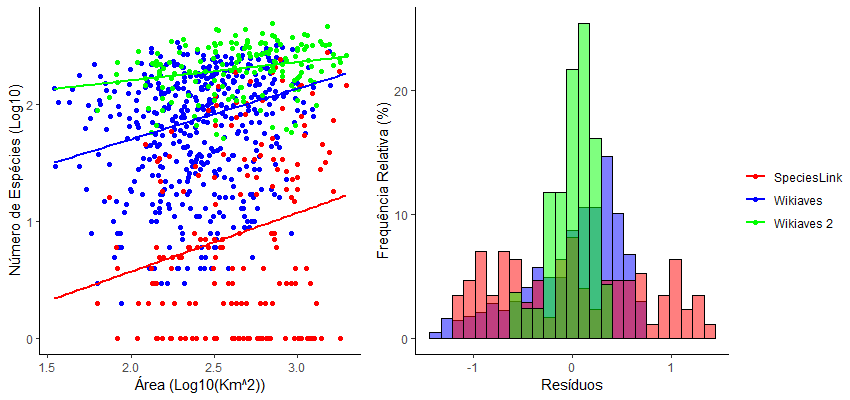
\includegraphics[width = 15cm]{Imagens/G07.png}
\\{\scriptsize Figura 14: Variação na quantidade de espécies das bases conforme aumento de área e resíduos. Foram excluídos, 19 outliers bivariados no Wikiaves, 9 no Wikiaves 2.}
\end{figure}

 \begin{resposta}
Quanto a quantidade de espécies os valores de $r$ diminuem no Wikiaves e aumentam no SpeciesLink, entretanto, não o suficiente para concluir que há ou não correlação linear entre as variáveis.

Tanto pelo gráfico quanto pelo modo com o qual os resíduos estão distribuídos identifica-se que não há correlação linear entre os dados. A situação não se altera ao se retirar os municípios excedentes. No geral, o tamanho de um município não possui grande influência em relação as variáveis resposta.
\end{resposta}

\subsubsection{População}

 \newpage

\begin{figure}[h!]
\centering
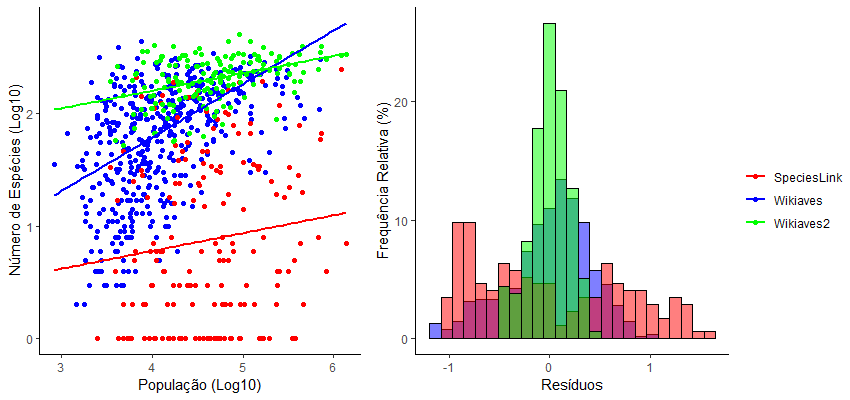
\includegraphics[width = 15cm]{Imagens/G08.png}
\\{\scriptsize Figura 15: Variação na quantidade de espécies das bases conforme aumento da quantidade de habitantes e resíduos. Foram excluídos, 19 outliers bivariados no Wikiaves, 14 no Wikiaves 2.}
\end{figure}

\begin{resposta}
De forma semelhante aos registros, a quantidade de espécies parece seguir o mesmo padrão. O valor de correlação é menor, percebe-se pelo gráfico que há relação para o Wikiaves. De fato, há um crescimento no Wikiaves, vez que, o SpeciesLink não segue padrão algum. Ao retirar os municípios excedentes o coeficiente angular da reta do Wikiaves aproxima-se de 0, ainda, é possível observar a relação.

Conclui-se que, este parâmetro influencia o Wikiaves, apenas. Ou seja, as bases de dados divergem quanto ao comportamento analisado nesta seção.
\end{resposta}

\subsubsection{Latitude}

 

\begin{figure}[h!]
\centering
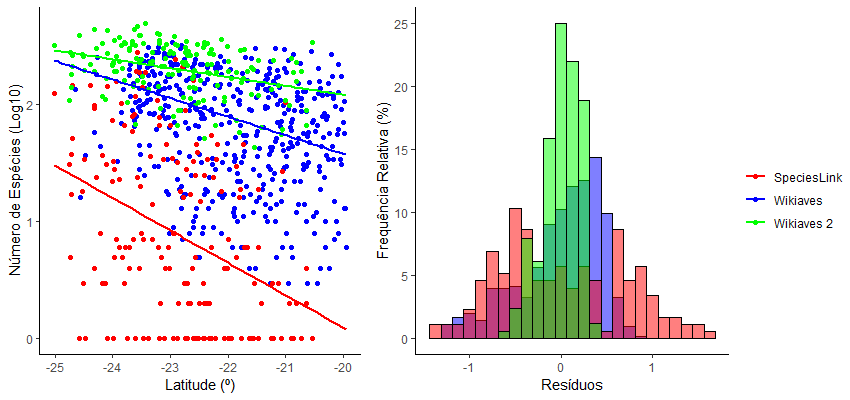
\includegraphics[width = 15cm]{Imagens/G09.png}
\\{\scriptsize Figura 16: Variação na quantidade de espécies das bases conforme aumento de latitude e resíduos. Foram excluídos, 26 outliers bivariados no Wikiaves, 9 no Wikiaves 2.}
\end{figure}

\begin{resposta}
Para a quantidade de espécies os bancos de dados apresentam valores próximos de $r$. Note o comportamento nos gráficos:

O valor dos resíduos no Wikiaves aumentam conforme aumento da altitude e, no SpeciesLink, ocorre o oposto. No geral, assume-se uma correlação fraca entre este fator e a quantidade de espécies. De fato, o mesmo vale para quando se retira os municípios com registro em apenas uma das bases.
\end{resposta}

\subsubsection{Longitude}

\begin{figure}[h!]
\centering
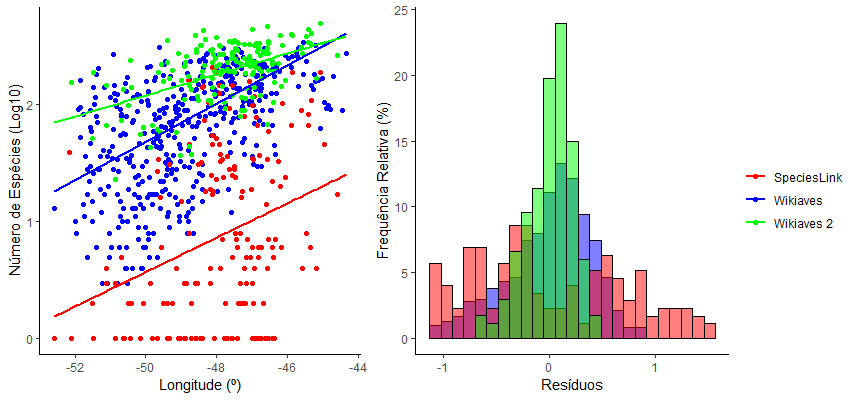
\includegraphics[width = 15cm]{Imagens/G10.png}
\\{\scriptsize Figura 17: Variação na quantidade de espécies das bases conforme aumento de longitude e resíduos. Foram excluídos, 29 outliers bivariados no Wikiaves, 6 no Wikiaves 2.}
\end{figure}

 \begin{resposta}
Novamente, os pares ordenados estão dispersos da linha de tendência, contudo, os quartis regulares e o crescimento são indícios de que há relação. Isso se mantém ao retirar os municípios com registro em apenas uma das bases.
\end{resposta}

\section{Wikiaves x SpeciesLink}

\hrulefill

Talvez a legenda da figura 20 tenha ficado muito grande.

\hrulefill


\begin{resposta}
Para relacionar as quantidades de registros e espécies dos bancos de dados, há de se dispor dos dados de forma diferente da apresentada anteriormente. A tabela (matriz) a seguir traz os valores de $p$ e $r$, respectivamente, acima e a abaixo da diagonal principal.
\end{resposta}

\newpage

\subsection{Registros}

\begin{figure}[h!]
\centering
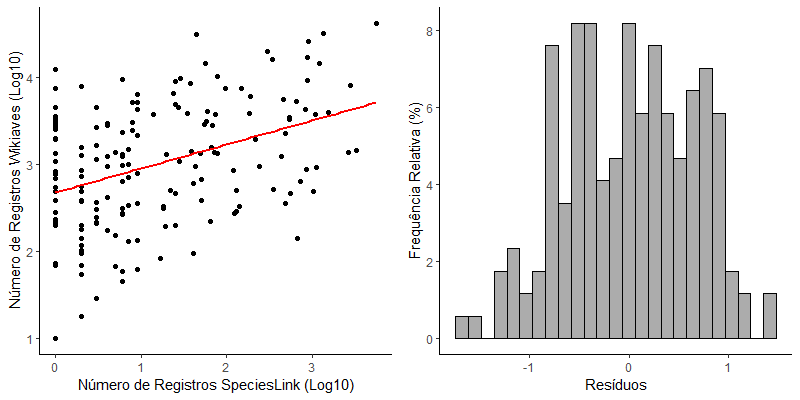
\includegraphics[width = 12cm]{Imagens/G11.png}
\\{\scriptsize  Figura 18: Número de registros no Wikiaves (Log10) por número de registros no SpeciesLink (Log10) e resíduos. Foram excluídos 2 outliers bivariados. Os valores de $n$,$r^2$ e $p$ são, respectivamente, $171$, $0,1588$ e $<0,0001$}
\end{figure}

\begin{resposta}
Pelos valores de $p$ expostos na tabela, os resultados experimentais possuem relação. Ao parear o log da quantidade de registros dos dois bancos de dados, obtém-se um coeficiente de correlação linear de 0,41. Este valor não é alto em comparação a outros que já obtidos, porém, o gráfico indica um crescimento linear.

Ao excluir os pares ordenados que geram resíduos discrepantes, há um aumento do valor de $p$ para $6,74*10^{-8}$ e uma diminuição de $r$ para $0,40$. Indicando que esses pares tem influência sob a curva.
\end{resposta}




\subsection{Espécies}

\begin{figure}[h!]
\centering
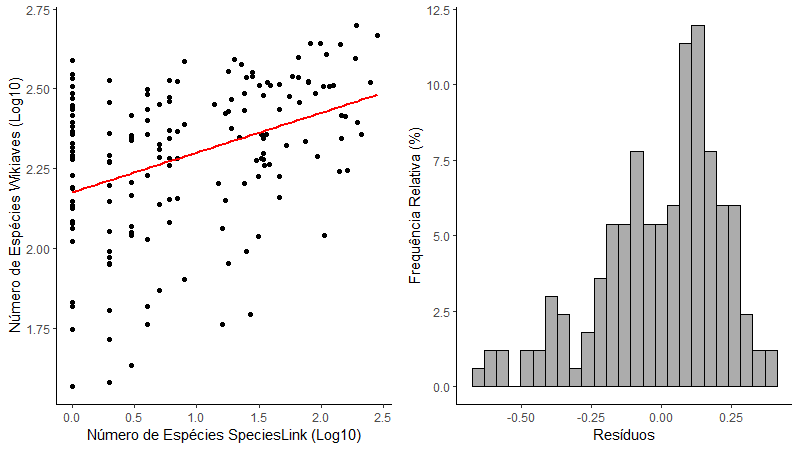
\includegraphics[width = 12cm]{Imagens/G12.png}
\\{\scriptsize Figura 19: Número de espécies no Wikiaves (Log10) por número de espécies no SpeciesLink (Log10) e resíduos. Foram excluídos 6 outliers bivariados. Os valores de $n$,$r^2$ e $p$ são, respectivamente, $167$, $0,1523$ e $<0,0001$}
\end{figure}

\begin{resposta}
Novamente, pelo valor $p$, é possível que haja relação entre os dados. O valor de $r$ é muito parecido com o anterior: $0,40$. Ou seja, a correlação linear é ligeiramente menor. Não obstante, no gráfico abaixo, nota-se que há uma correlação linear. 

\end{resposta}

\subsection {Registros x Espécies}

\begin{figure}[h!]
\centering
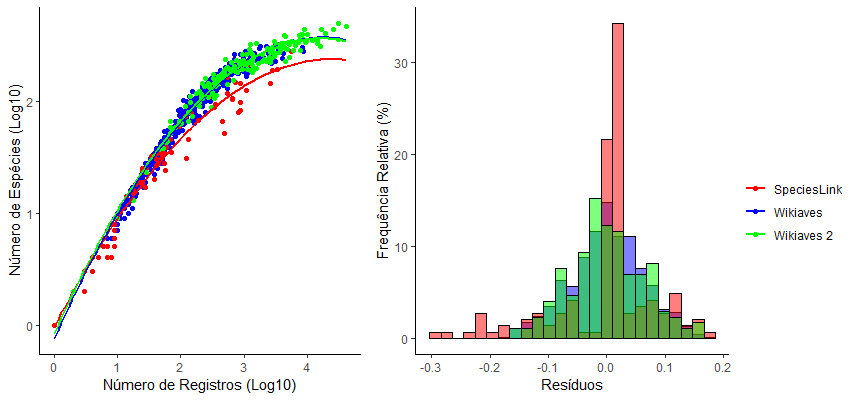
\includegraphics[width = 15cm]{Imagens/G13.png}
\\{\scriptsize Figura 20: Quantidade de espécies x Quantidade de registros. Modelo não linear. Foram excluídos 11 outliers bivariados no Wikiaves, 30 no SpeciesLink e 2 no Wikiaves 2.  Os valores de $n$,$r^2$ e $p$ são, respectivamente, $620$, $0,9875$ e $<0,0001$; $143$, $0,9867$ e $<0,0001$ no SpeciesLink; $171$, $0,9647$ e $<0,0001$ no Wikiaves 2. }
\label{Figura 20}
\end{figure}

\begin{resposta}
Até o momento, os valores de $r$ são os maiores encontrados: para o Wikiaves $0,91$ e para o SpeciesLink $0,94$. Porém, o gráfico traz fortes indicativos de que a correlação não é linear.

Portanto, ao assumir que a correlação não é linear obtemos aproximações mais exatas para as curvas, nestas os valores de $r^2$ são de $0,9604$ no Wikiaves e $0,9067$ no SpeciesLink, isto é, os valores próximos de 1 indicam que há forte correlação nas aproximações abaixo.

É possível, ainda, otimizar estes valores ao retirar os resíduos discrepantes. No Wikiaves, há um leve aumento de $r^2$ para $0,9647$.


\end{resposta}


\section{Mapas}

\hrulefill

Estou tentando configurar algumas coisas nos mapas, mas isto é mais uma questão minha com o R do que de conteúdo em si, note que, na figura 25, não há nenhum município com 1 única espécie no WAV2, então o programa \asp{pula} uma classe com isso, dá pra confundir com o SpeciesLink que está uma classe abaixo. Como é uma questão técnica acredito que consigo resolver isto tranquilamente.

Eu intercalei a forma como mostrar os mapas nas figuras 24 e 25, matriz com WAV em cima e SPL e legenda em baixo ou matriz com WAV à direita e SPL e legenda à esquerda. Não sei se a legenda ficou boa do jeito que está, mas desse modo economiza espaço.

\hrulefill

\begin{resposta}
Os mapas facilitam a observação espacial dos fatores abordados na seção 2. Ademais, possibilitam a observação de como se distribuem os registros ou espécies em cada banco de dados pelo estado de São Paulo. A cada subseção serão mostrados mapas de acordo com os devidos temas.
\end{resposta}

\subsection{Altitude}

\begin{figure}[h!]
\centering
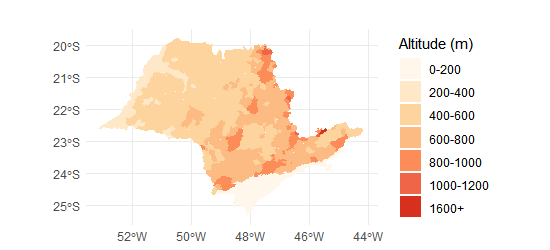
\includegraphics[height = 5cm]{Imagens/M01.png}
\\{\scriptsize Figura 21: Distribuição de altitude (em metros) no estado de São Paulo.}
\end{figure}

\begin{resposta}
A distribuição de altitude no estado se dá de maneira regular. Ainda, a maior parte dos municípios se apresenta em uma faixa específica dentre os valores determinados.
\end{resposta}

\subsection {Área}

\begin{figure}[h!]
\centering
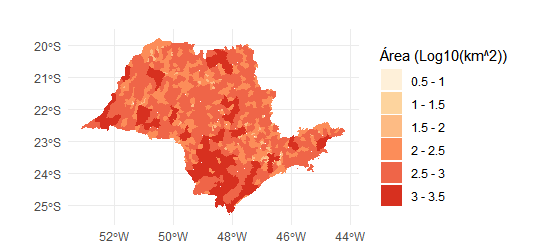
\includegraphics[height = 5cm]{Imagens/M02.png}
\\{\scriptsize Figura 22: Distribuição de área (em $Log_{10}Km^2$) no estado de São Paulo.}
\end{figure}

\begin{resposta}
A distribuição do $\log_{10}$ da área, também é regular. Há uma quantidade limitada de municípios com áreas muito baixas, ou seja, os outliers.
\end{resposta}


\subsection {População}

\newpage

\begin{figure}[h!]
\centering
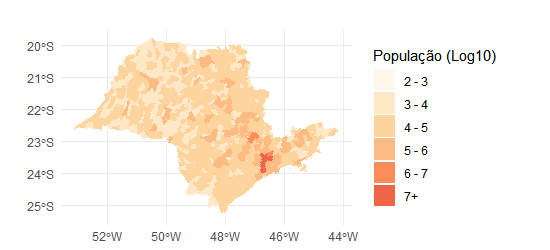
\includegraphics[height = 5cm]{Imagens/M03.png}
\\{\scriptsize Figura 23: Distribuição de densidade populacional no estado de São Paulo.}
\end{figure}

\begin{resposta}
A distribuição do $\log_{10}$ da população também é regular, a cidade de São Paulo é um outlier evidente no mapa.
\end{resposta}

\subsection {Registros}

\begin{figure}[h!]
\centering
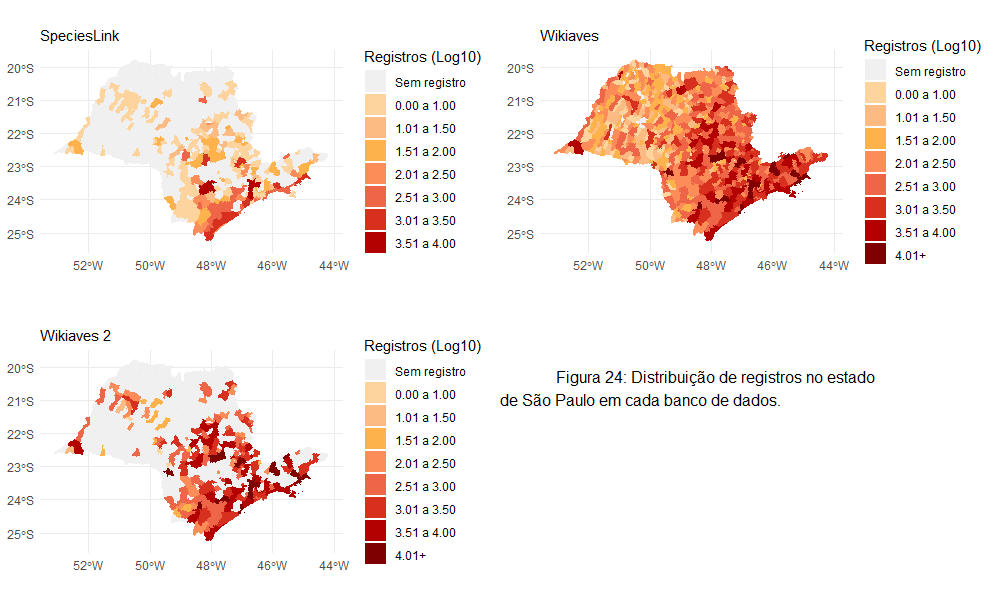
\includegraphics[width=17cm]{Imagens/M04.png}
\end{figure}

\begin{resposta}
Há uma desigualdade perceptível entre os bancos de dados quanto a distribuição espacial da quantidade de registros. O mapa do Wikiaves é mais saturado que o do SpeciesLink, a quantidade de cidades sem registro, também, torna-se ainda mais evidente: enquanto o Wikiaves cobre quase todo o estado, o SpeciesLink não cobre metade disto. 

Não obstante, há similaridades observadas nos mapas, eles mostram uma expressão mais forte no litoral e, conforme se movimenta para  o interior há uma diminuição na quantidade de registros, enfatizando a relevância dos parâmetros de latitude e longitude.
\end{resposta}

\subsection {Espécies}

\begin{figure}[h!]
\centering
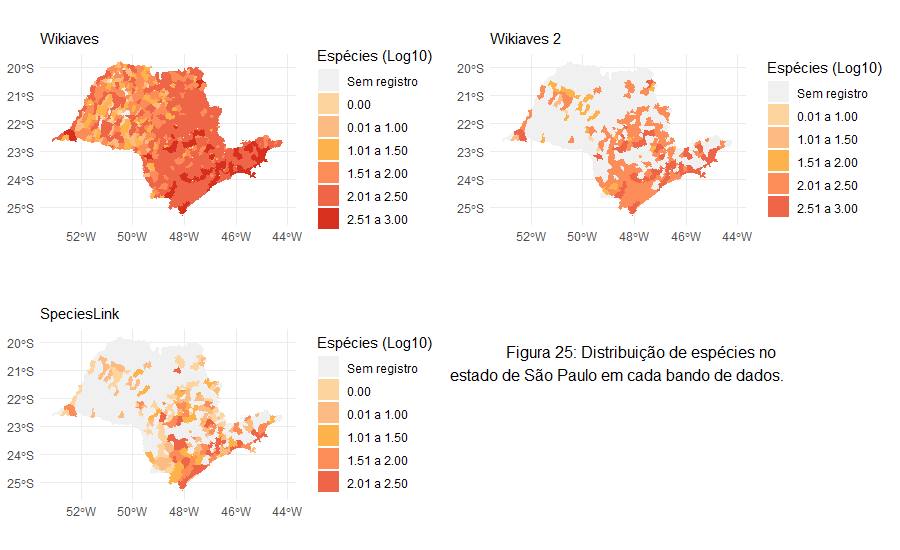
\includegraphics[width=17cm]{Imagens/M05.png}
\end{figure}

\begin{resposta}
As mesmas divergências e semelhanças mencionadas na subseção anterior são encontradas para a quantidade de espécies, de forma menos chamativa. 
\end{resposta}


\section{Análise multivariada}

Pela terceira vez estou te mandando um rascunho dessa parte de análise multivariada (peço desculpas). Eu vou dividir em duas partes aqui porque \textbf{por enquanto} é o que faz sentido para mim, embora essas 2 partes se unem ao final.



\subsection{Registros/Espécies}

Para as espécies, acho que não muda muito do que eu já estava fazendo que é a matriz de distância e o cluster. Acredito que um cluster hierárquico aglomerativo, isto é, dendrograma é uma boa opção para nosso tipo de análise (Greenacre), o principal problema disto é decidir onde deve ser feito o \asp{corte} para que o dendrograma seja interpretável, o senhor havia comentado que dá pra fazer isto de acordo com a figura 20. Pergunto se o corte tem que ser igual nos bancos de dados, digo, se for utilizada a quantidade de registros = 100 haverá muito mais \asp{pontos} em WAV2 em relação ao SPL. 

Uma vez construído o dendrograma (dessa vez de um modo sério e não só para eu me habituar a eles em R), o Borcard passa para uma análise de \asp{cophonetic correlation}, não pesquisei detalhes sobre isso, afinal, se formos fazer uma análise do tipo será posterior ao dendrograma (eu nem sei se ela é interessante para nossos propósitos, do que entendo ela está na área de \asp{supervised learning}, o Borcard não chega a colocar deste modo contudo, do que entendi o que ele coloca como \asp{cross validation} é como a ideia de test e training sets). 

\subsection{Variáveis Explanatórias}

O senhor também falou para agrupar as variáveis explanatórias, para tanto, utiliza-se não uma matriz de distância, porém, uma matriz de correlação (Gotelli, Valentin). Para mim, o que faria sentido nesse tipo de matriz é testar a \asp{multi-normalidade} (não sei se este é o termo correto) para partir para uma regressão múltipla. 

Da regressão múltipla da para partir para o capítulo 4, seção 11 do Borcard, que diz respeito a \asp{Multivariate Regression Trees}. É outra coisa que eu não aprofundei meus estudos, mas, se formos fazer isto ainda há um grande caminho a ser trilhado. E esta é a última coisa que o autor introduz antes de entrar na parte de ordenação, então acho que ficaria por aqui.

\subsection{Geral}

Não sei em que momento o teste de mantel entraria nessa história toda, acredito que está ligado à Cophenetic correlation, mas, como não estudei isto a fundo posso estar completamente errada. Os biomas devem entrar na parte de variáveis explanatórias.

Se este esboço estiver mais ou menos correto, podemos dividir isto em partes? Digo, há a ANOVA (não sei se haverá MANOVA), a análise de objetos e a de descritores. Se pudermos dividir em partes peço que me diga por qual das 3 começar. Se este esboço não estiver correto, começarei pela ANOVA que creio ser independente da parte de análise multivariada.



%\newpage
%\appendix


\end{document}
